\chapter[Fundamentos de condução de calor]{Fundamentos de condução de calor: Equações governantes e condições de contorno}

\section{Fluxo de Calor e Temperatura}

A condução de calor pode ser entendida como a transferência de energia das partículas mais energizadas para as menos energizadas de um determinado corpo. Esta transferência se dá pela interação molecular. Este fenômeno, por sua vez pode acontecer quer o corpo seja sólido, líquido ou gasoso, embora, nos sólidos ela seja mais eficiente. Esta é, portanto, a razão pela qual este texto somente tratará da condução de calor em sólidos.

Assim, em um corpo sólido cuja variação de temperatura esteja presente, a taxa de transferência de calor por condução ocorrerá da região de alta temperatura para a região de baixa temperatura.  Neste texto, a  \textit{transferência de calor} será tratada como taxa de calor dado em Joules por segundo $[J/s]$ enquanto o termo \textit{fluxo de calor} será associado à taxa de calor por unidade de área  $[W/m^2]$. Ambos os termos estão associados à energia vibracional dos átomos e molécula do corpo.

O fluxo de calor não pode ser medido diretamente.  Entretanto, os efeitos do fluxo de calor podem ser sentidos através da observação. Por exemplo, o aquecimento de uma placa exposta ao sol, o derretimento de uma pedra de gelo, o aquecimento de uma panela ao fogo ou ainda o aquecimento da água no interior da panela. São inúmeros os exemplos. A troca de calor por condução foi investigada pelo pesquisador francês Joseph Fourier cuja observação experimental estabeleceu que a taxa  calor por condução através de uma superfície é dada pelo vetor $\vec{q}$ e pode ser escrita como
\begin{equation}\label{eq:vetorFluxoCalor}
	\vec{q}= -kA \frac{\partial{T}}{\partial{x}} \vec{i} 
	-kA \frac{\partial{T}}{\partial{y}} \vec{j}
	-kA \frac{\partial{T}}{\partial{z}} \vec{k} 
\end{equation}
onde o parâmetro $k$ é a condutividade térmica com unidades $W/(m K)$. Em geral, a condutividade térmica pode ser uma função da temperatura. O sinal negativo implica que o fluxo de calor (que sempre flui no sentido da redução da temperatura) será positivo (por convenção) no sentido do crescimento do eixo. Isso ocorrerá em qualquer das componentes nas direções, seja x, y ou z, ou seja 
\begin{equation}\label{eq:componentesFluxoCalor}
	q_x = -kA \frac{\partial{T}}{\partial{x}}; 
	\qquad  q_y = -kA \frac{\partial{T}}{\partial{y}}; 
	\qquad  q_z = -kA \frac{\partial{T}}{\partial{z}}   
\end{equation}
Esta é a lei de Fourier para a condução de calor. A lei de Fourier se aplica a qualquer corpo que seja homogêneo (possua a mesma substância o tempo todo), isotrópico (o calor flui igualmente em qualquer direção) e com tamanho em macroescala (não muito pequeno).

\section{Equação diferencial geral da difusão de calor} 

\subsection{Equação da difusão de calor diferencial em coordenadas retangulares} 

A equação da difusão de calor é obtida nesta seção para corpos isotrópicos cuja condutividade térmica é constante espacialmente. Além disso, $k$ também não varia com a temperatura. Ou sejam trataremos de problemas lineares. O sistema de coordenadas retangulares $(x; y; z)$ é usado. Obtém-se a equação da difusão de calor aplicando-se o princípio da conservação de energia em uma determinada região de estudo.

Observa-se na  Fig.~\ref{fig:balanco} que um corpo em forma de paralelepípedo tem em suas superfícies informações de temperaturas, $T_{1}$, e $T_{2}$, meios fluídos representados por $h$ e $T_{\infty}$ ou fluxo de calor impostos $q''_0$ e $q''_1$. Essas informações, serão abordadas na próxima seção e representam de fato as condições de contorno do problema a ser analisado.

Um caminho visando a obtenção do campo de temperatura no interior de um sólido, é  a aplicação do princípio de conservação de energia nesse corpo. Entretanto, a aplicação desse princípio exige que ele se dê em uma região de estudo (sistema ou volume de controle) cujas propriedades sejam constantes. Assim, considerando que no problema representado pela Fig.~\ref{fig:balanco} existem gradientes de temperatura no corpo, a primeira lei da termodinâmica só poderá ser aplicada se esta região representar um volume de controle infinitesimal. Esse volume infinitesimal está localizado na coordenada $(x, y, z)$ no corpo e possui um volume $dV = dx dy dz$ conforme mostrado na Fig.~\ref{fig:balanco}. 

Nesse caso, considerando um instante $t$ qualquer, ao aplicar-se o balanço de energia, obtém-se
\begin{figure}[ht]
	\centering
	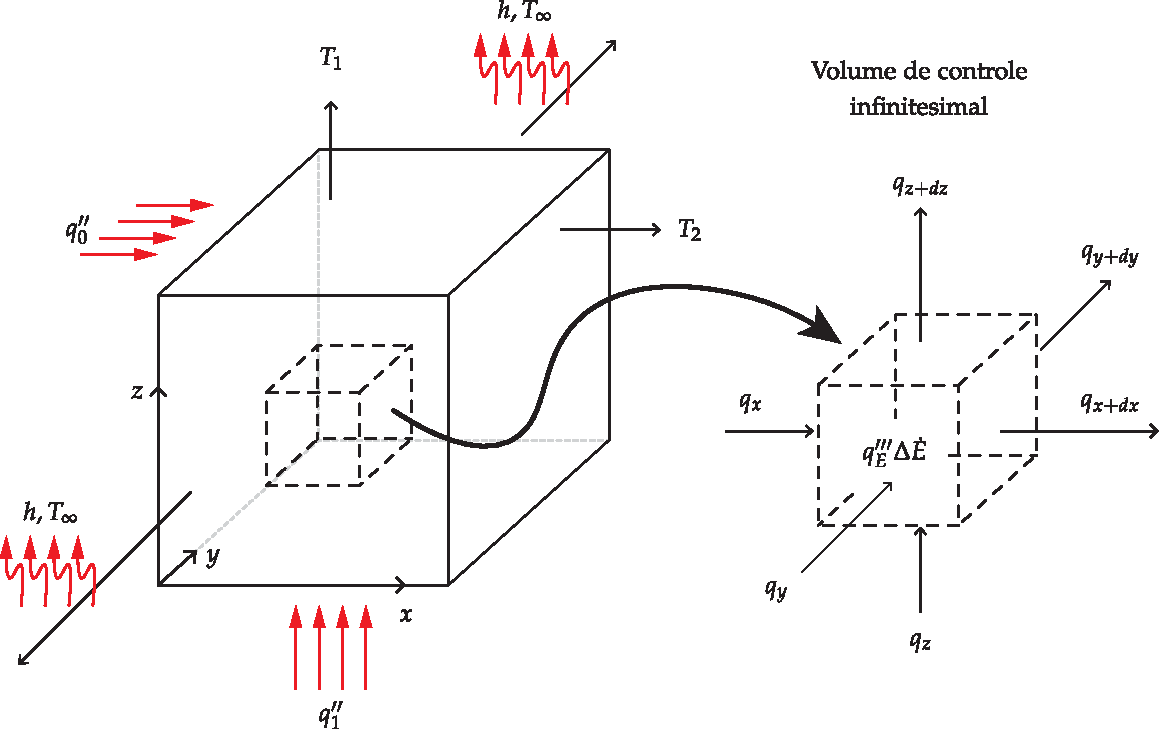
\includegraphics[scale=0.7]{figuras/cap1/balancoEnergia.pdf}
	\caption{Balanço de energia em um volume de controle infinitesimal}	
	\label{fig:balanco}
\end{figure}
\begin{equation}\label{eq:qct}	
	(q_x - q_{x + dx}) +
	(q_y - q_{y + dy}) +
	(q_z - q_{z + dz}) + 
	g(x,y,z,t)  \; dx \; dy \; dz = 
	\rho \; dx \; dy \; dz \; c \; \frac{\partial T}{\partial t}
\end{equation}
Observemos separadamente cada termo da Eq. (\ref{eq:qct}).

\begin{itemize}
	\item Taxa líquida de fluxo de calor entrando e saindo das seis faces do volume de controle.
	\item Consideremos  a convenção de que o fluxo de calor seja positivo nas direções de coordenadas positivas.
	\item A taxa de fluxo líquido de calor é a diferença entre a taxa de fluxo de entrada e a taxa de saída, ou seja
\end{itemize}
\begin{equation}\label{eq:qliq}	 
	q_{\text{liq}} = (q_x - q_{x + dx}) + (q_y - q_{y + dy}) + (q_z - q_{z + dz})
\end{equation}

Observe, por exemplo, que a taxa de fluxo de calor por condução entra no V.C. na face $x$ e sai na face em $x + dx$. Esta taxa é proporcional a área perpendicular a essa direção.  

Nota-se, entretanto, que a posição $x + dx$ corresponde a uma posição muita próxima $x$, porém é de valor simbólico devido o infinitésimo $dx$. Nesse caso, é conveniente que seu cálculo se dê em função da variável exata $x$. Como os pontos situam-se muito próximos, pode-se avaliar a posição $x + dx$ em torno de $x$ usando-se a aproximação em série de Taylor truncada no segundo termo, ou seja, 
\begin{equation}\label{eq:dif1}
	q_{x + dx} = q_x + \frac{\partial q_x}{\partial x} dx 
\end{equation}
\begin{figure}[!ht]
	\centering
	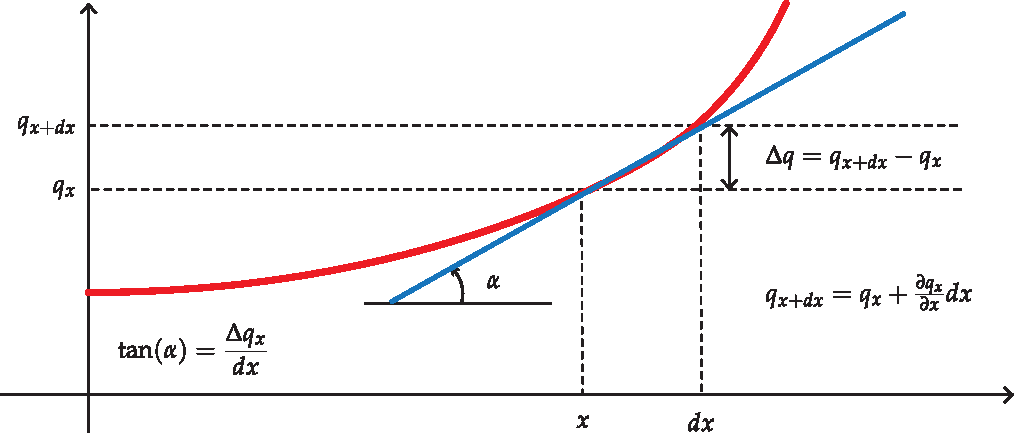
\includegraphics[scale=0.9]{figuras/cap1/aproximacaoTaylor.pdf}
	\caption{Aproximação de Taylor}
	\label{fig:Taylor}
\end{figure} 
A Figura~\ref{fig:Taylor} representa geometricamente esta aproximação, cujo valor de $\partial q_x /\partial x$ tende exatamente ao valor da derivada no ponto $x$ da curva dada pela funçao $q_x$. Assim, analogamente pode-se escrever para as direções $y$ e $z$
\begin{equation}\label{eq:dif2}
	q_{y + dy} = q_y + \frac{\partial q_y}{\partial y} dy  \qquad \text{e}
\end{equation}
\begin{equation}\label{eq:dif3}	
	q_{z + dz} = q_z + \frac{\partial q_z}{\partial z} dz 
\end{equation}

Substituindo as Eqs.(\ref{eq:dif1}),  (\ref{eq:dif2}) e (\ref{eq:dif3}) na Eq. (\ref{eq:qliq}) obtém-se
\begin{equation}
	q_{\text{liq}} =
	- \frac{\partial q_x}{\partial x} dx 
	- \frac{\partial q_y}{\partial y} dy 
	- \frac{\partial q_z}{\partial z} dz 
\end{equation}

Substituindo a definição de cada componente de taxa de fluxo de calor por condução das pelas Eqs.~\ref{eq:componentesFluxoCalor} em suas respectivas direções obtém-se

\begin{equation}
	q_{\text{liq}}=
	- \frac{\partial}{\partial x} \left( - k A_x \frac{\partial T}{\partial x} \right) 
	- \frac{\partial}{\partial y} \left( - k A_y \frac{\partial T}{\partial y} \right)  
	- \frac{\partial}{\partial z} \left( - k A_z \frac{\partial T}{\partial z} \right)   
\end{equation}
onde $A_x, A_y, A_z$ representam as áreas perpendiculares às respectivas direções $x, y, z$. Portanto, pode-se escrever
\begin{equation}\label{eq:Fourierdif1}
	q_{\text{liq}}=
	- \frac{\partial}{\partial x} \left( - k\;dy\;dz \frac{\partial T}{\partial x} \right)  
	- \frac{\partial}{\partial y} \left( - k\;dx\;dz \frac{\partial T}{\partial y} \right)  
	- \frac{\partial}{\partial z} \left( - k\;dx\;dy \frac{\partial T}{\partial z} \right)  
\end{equation}

Apresentam-se no final desta capítulo algumas observações sobre a Lei de Fourier. Considerações sobre o sinal negativo, a sua aplicação em meios macroscópio e aspectos microscópicos bem como as características da condutividade térmica em meios isotrópicos e anisotrópicos.

\textbf{Taxa de geração de energia.} A geração de energia é a energia que afeta o temperatura em todo o volume do corpo. Distingue-se da energia que entra no corpo através dos limites de suas superfícies. A geração de energia pode vir do aquecimento da resistência elétrica dentro do corpo (Efeito Joule), da reação de alguns elementos químicos (por exemplo, o concreto gera calor durante a cura) ou da absorção de radiação (nuclear, micro-ondas ou outra energia eletromagnética). A geração de energia pode variar de um ponto a outro no interior do corpo assim como pode variar com o tempo. A geração de energia também pode ser simplesmente igual a zero. É dado, nesse texto, o símbolo $g(x, y, z, t)$ com unidades $W/m^3$ (taxa de geração de energia por unidade de volume). Assim, considerando o volume de controle infinitesimal tem-se,	
\begin{equation}
	\label{eq:qg}	
	\text{(Taxa de geração de energia)}=g(x,y,z,t) \;dx \;dy \;dz
\end{equation}

\textbf{Taxa de armazenamento de energia.} Uma mudança no armazenamento de energia é definida por $c \Delta T$ para corpos sólidos. Aqui $c$ é o calor específico, J/(kg K), e $\Delta T$ é a variação de temperatura. A taxa de armazenamento de energia específica (por unidade de massa) é dada pela derivada temporal $c(\partial T / \partial t)$. A derivada parcial no tempo é usada porque $T$ também depende da posição $(x,y,z)$. Multiplique a taxa de variação temporal da energia interna específica pela densidade e pelo volume para obter Watts: 
\begin{equation}\label{eq:qct1}	
	\text{(Taxa de armazenamento de energia)} = \rho c \; \frac{ \partial T} {\partial t} \;dx \;dy \;dz
\end{equation}
Assim, substituindo a Eq.(\ref{eq:Fourierdif1}) na equação de energia ( Eq. \ref{eq:qct}) obtém-se 

\begin{equation}\label{eq3Da}
	\frac{\partial}{\partial x} \left(k\frac{\partial T}{\partial x}\right) + 
	\frac{\partial}{\partial y} \left(k\frac{\partial T}{\partial y}\right) + 
	\frac{\partial}{\partial z} \left(k\frac{\partial T}{\partial z}\right) + 
	g(x,y,z,t) = \rho c \frac{\partial T}{\partial t}  
\end{equation}	
e no caso especial em que a condutividade térmica não depende da posição (meios isotrópicos) obtém-se
\begin{equation}\label{eq3Db}
	\frac{\partial^2 T}{\partial x^2} +
	\frac{\partial^2 T}{\partial y^2} + 
	\frac{\partial^2 T}{\partial z^2} = 
	\frac{1}{\alpha} \frac{\partial T}{\partial t}  
\end{equation}
onde $\alpha = k/(\rho c)$ é a difusividade térmica $[m^2/s]$.

\subsection{Outros sistemas de coordenadas}

A equação da energia pode ser aplicada em outros sistemas de coordenadas ortogonais como  os sistemas cilíndrico e esférico apresentados nas Figs.~\ref{fig:coordCilindricas}-\ref{fig:coordEsfericas}.

Uma forma direta de se obter a Equação da Difusão em outras coordenadas é a aplicação da equação de Fourier em sua forma vetorial na equação da energia.

Assim, se a forma vetorial da lei de Fourier é dada por
\begin{equation}\label{eq:Fourier0}
	\mathbf{q} = - k \nabla T  
\end{equation}
onde $\nabla T$ é o gradiente de temperatura e $\mathbf{q}$ é o vetor de fluxo de calor.

Uma forma vetorial da equação de energia que é independente do sistema de coordenadas pode ser dada por
\begin{equation}\label{eq:Fourier}
		- \nabla \cdot \mathbf{q} + g(\mathbf{r},t) = \rho c \frac {\partial T} {\partial t}
\end{equation}
onde $\nabla \cdot \mathbf{q}$ é a divergência do fluxo de calor. A equação da energia em qualquer sistema dado pode ser encontrado substituindo a forma correta da divergência e operadores de gradiente para esse sistema de coordenadas específico. Para uma derivação mais detalhada, consulte \textcite[p. 36]{ozisik1993}.

\subsubsection{Sistema de Coordenadas Cilíndricas}
	
No sistema de coordenadas cilíndricas mostrado na Fig.~\ref{fig:coordCilindricas} a equação da energia é dada por
	
\begin{figure}[ht]
	\centering
	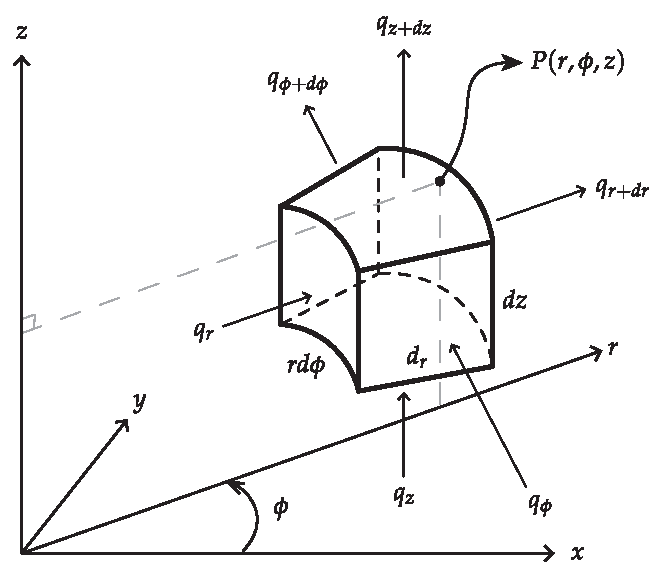
\includegraphics[scale=.9]{figuras/cap1/coordenadasCilindricas.pdf}
	\caption{Sistema de coordenadas cilíndricas e representação do volume de controle  infinitesimal}
	\label{fig:coordCilindricas}
\end{figure}
\begin{equation}\label{eq3Dcila}
	\frac{1}{r}	\frac{\partial}{\partial r} \left(kr\frac{\partial T}{\partial r}\right) +
	\frac{1}{r^2} \frac{\partial}{\partial \phi} \left(k\frac{\partial T}{\partial \phi}\right) + \frac{\partial}{\partial z}\left(k\frac{\partial T}{\partial z}\right) + g = 
	\rho c \frac{\partial T}{\partial t}  
\end{equation}	
	
Considerando $k$ constante obtém-se,
\begin{equation}\label{eq3Dcilb}
	\frac{\partial ^2T}{\partial r^2} + 
	\frac{1}{r} \frac{\partial T}{\partial r} + 
	\frac{1}{r^2} \frac{ \partial ^2T} {\partial \phi ^2} +
	\frac{\partial ^2T}{\partial z^2} + \frac{g}{k} = 
	\frac{1}{\alpha} \frac{\partial T}{\partial t}  
\end{equation}	
	
\subsubsection{Sistema de Coordenadas esféricas}
	
Analogamente, no sistema de coordenadas esféricas mostrado na Fig.~\ref{fig:coordEsfericas}, a equação da energia é dada por
\begin{figure}[ht]
	\centering
	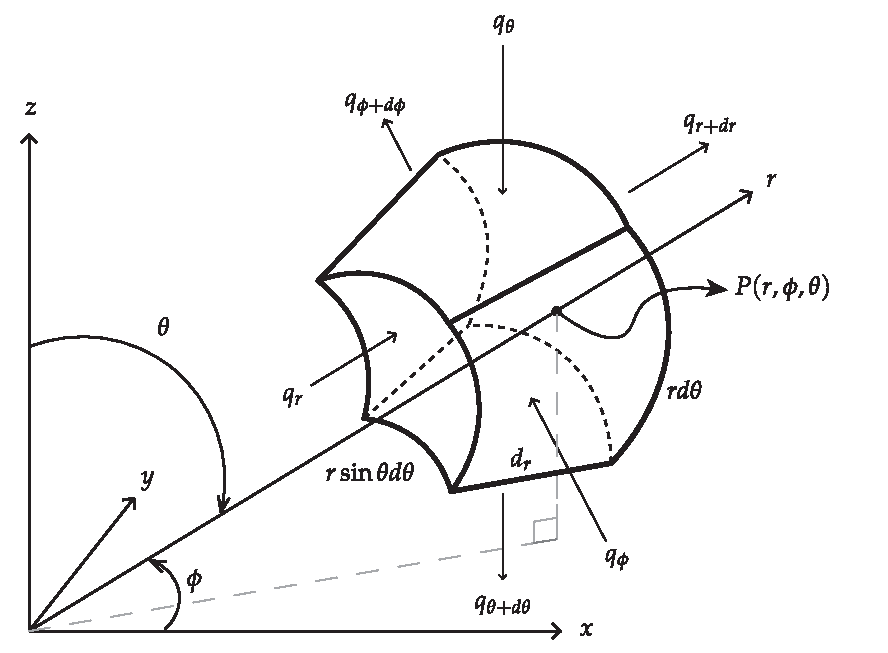
\includegraphics[scale=.9]{figuras/cap1/coordenadasEsfericas.pdf}
	\caption{Sistema de coordenadas esféricas e representação do volume de controle infinitesimal }
	\label{fig:coordEsfericas}
\end{figure} 

\begin{equation}\label{eq3Desfa}
	\frac{1}{r^2} \frac{\partial}{\partial r} 
	\left(kr^2\frac{\partial T}{\partial r}\right) +
	\frac{1}{r^2\sin\theta} \frac{\partial}{\partial\theta} 
	\left(k\sin\theta\frac{\partial T}{\partial\theta}\right) +
	\frac{1}{r^2\sin\theta} \frac{\partial}{\partial\theta} 
	\left(k\sin^2\theta\frac{\partial T}{\partial\phi}\right) + 
	g = \rho c \frac{\partial T}{\partial t}  
\end{equation}	

Similarmente, se $k$ não varia com a posição, obtém-se
\begin{equation}\label{eq3Desfb}
	\frac{1}{r} \frac{\partial^2\left(rT\right)}{\partial r^2} +
	\frac{1}{r^2\sin\theta} \frac{\partial}{\partial\theta}
	\left(\sin\theta\frac{\partial T}{\partial\theta}\right) + 
	\frac{1}{r^2\sin^2\theta}\frac{\partial^2 T}{\partial\phi^2} + 
	\frac{g}{k} = \frac{1}{\alpha}\frac{\partial T}{\partial t}  
\end{equation}
	
\subsection{Condições particulares}
Este curso trata de soluções para a equação de energia conforme elas se aplicam a problemas de engenharia e física. As soluções únicas de cada problema  são estabelecidas pela solução geral aplicando-se as condições de contorno específicas, ou seja, o valor da temperatura (ou sua derivada) nos limites do corpo sólido. A combinação da equação de energia, das condições de contorno específicas e da condição inicial é chamada de problema de valor de contorno. A maior parte deste livro trata de corpos com geometria que possam ser descritos por coordenadas ortogonais. Ou seja, cujos limites estejam localizados onde uma coordenada é uma constante.
	
O número de condições de contorno para um problema de valor de contorno depende da forma da equação de energia e da geometria do sistema em consideração. Por exemplo, a equação de energia bidimensional no sistema de coordenadas retangulares,
\begin{equation}\label{eq2D}
	\frac{\partial ^2T}{\partial x^2} +
	\frac{\partial ^2T}{\partial y^2} + 
	\frac{g(x,y,z,t)}{k} = \frac{1}{\alpha} \frac{\partial T}{\partial t}  
\end{equation}
requer cinco condições: duas para cada um dos limites em $x$ e $y$ e uma condição inicial. As condições de contorno normalmente têm a forma	
\begin{equation}
		k_i \frac{ \partial T} {\partial \eta_i}  +h_i T =  f_i (r_i,t)   
\end{equation}
onde todas as quantidades são avaliadas no limite $i \; esimo$. Aqui $r_i$ é a localização do limite $i \; esimo $ em um sistema de coordenadas específico e $\eta_i$ é o vetor normal da unidade externa no limite. 

As condições iniciais têm a forma
\begin{equation}
	T(r_i, t=0) = F(r_i)   
\end{equation}

As condições de contorno e as condições iniciais são discutidas em detalhes na próxima seção.

\section{Condições de contorno e condição inicial}	

\subsection{Condição de contorno do primeiro tipo}
A Figura \ref{fig:ccTemperaturaPrescrita} apresenta a condição de contorno, chamada do \textit{primeiro tipo}, em que a temperatura da superfície é conhecida. No exemplo apresentado, a temperatura $T_s$ é conhecida e portanto tem-se uma temperatura prescrita. Em alguns textos clássicos, esta condição é também chamada de condição de \textit{Dirichilet}.
\begin{equation}\label{eq:q01}
	T(x=0,t) = T_s 
\end{equation}

\begin{figure}[H]
	\centering
	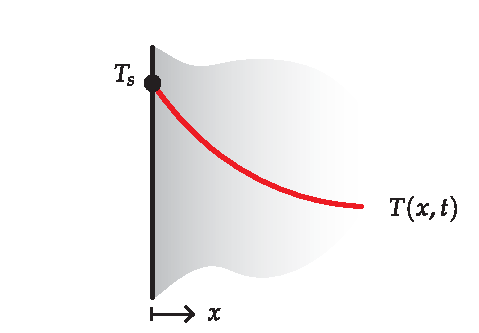
\includegraphics[scale=1]{figuras/cap1/ccTemperaturaConstante}
	\caption{Condição de contorno do primeiro tipo: temperatura prescrita, $T_s$}
	\label{fig:ccTemperaturaPrescrita}
\end{figure}

\subsection{Condição de contorno do segundo tipo}
A Figura \ref{fig:ccFluxoCalor} por sua vez se refere à condição de contorno do \textit{segundo tipo}, sendo nesse caso, conhecido o fluxo de calor no respectivo contorno. Como a informação direta da temperatura não está disponível, a informação desejada para a solução da equação diferencial deve ser obtida através de um balanço de energia na respectiva superfície, ou seja
\begin{equation}\label{eq:q1}
+ q''_s A - q_n = 0  
\end{equation}
Logo,
\begin{equation}\label{eq:q2}
q_n = -k A\left.{\frac{\partial{T}}{\partial{x}}}\right|_{x=0} = q''_s A 
\end{equation}
ou seja,
\begin{equation}\label{eq:q3}
-k\left.{\frac{\partial{T}}{\partial{x}}}\right|_{x=0} = q''_s  
\end{equation}
\begin{figure}[H]
	\centering
	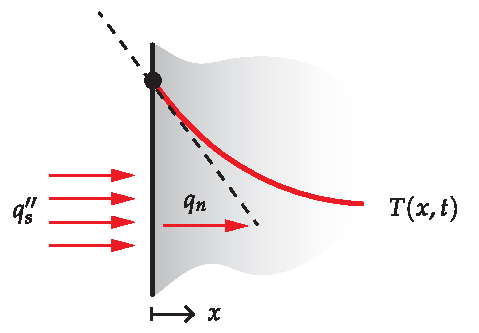
\includegraphics[scale=1]{figuras/cap1/ccFluxoConstante}
	\caption{Condição de contorno do segundo tipo: fluxo de calor prescrito, $q''_0$}
	\label{fig:ccFluxoCalor}
\end{figure}

Caso a superfície esteja isolada termicamente (\hl{fronteita adiabática}), como mostra a Fig.~\ref{fig:ccIsolado}, então pode-se escrever
\begin{equation}\label{eq:q4}
-k\left.{\frac{\partial{T}}{\partial{x}}}\right|_{x=0} =0
\end{equation}

\begin{figure}[H]
	\centering
	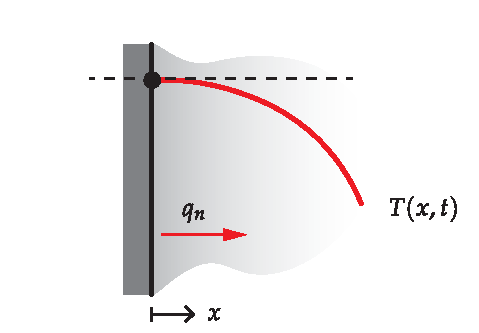
\includegraphics[scale=1]{figuras/cap1/ccAdiabatica}
	\caption{Condição de contorno do segundo tipo: isolado}
	\label{fig:ccIsolado}
\end{figure}

Em alguns textos clássicos, esta condição é também chamada de condição de \textit{Neumann}.

\subsection{Condição de contorno do terceiro tipo}
A condição de contorno do terceiro tipo representada pela Fig.~\ref{fig:ccConveccao} diz respeito à superfície estar exposta a um meio convectivo. 

Nesse caso, um balanço de calor na superfície é escrito como
\begin{equation}\label{eq:q5}
+ q_h - q_n = 0 \Rightarrow q_n = q_h \qquad \text{e}
\end{equation}
\begin{equation}\label{eq:q6}
	-k\left.{\frac{\partial{T}}{\partial{x}}}\right|_{x=0} 
	= h A (T_{\infty} - T(x=0,t))
\end{equation}

\begin{figure}[H]
	\centering
	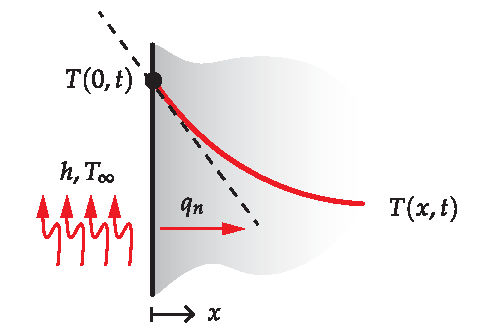
\includegraphics[scale=1]{figuras/cap1/ccConveccao}
	\caption{Condição de contorno do terceiro tipo: face exposta a um meio convectivo}
	\label{fig:ccConveccao}
\end{figure}

Em alguns textos clássicos, esta condição é também chamada de condição de \textit{Robin} ou condição convectiva. 

É importante destacar que ao se aplicar o balanço de energia na superfície, o sinal $+$ indica que a taxa de calor chega na superfície, enquanto o sinal $-$ indica que a taxa de calor deixa a superfície. Como o balanço de energia na superfície, não envolve nenhum fenômeno volumétrico, este balanço sempre será nulo, independente se o problema analisado em questão for transiente ou não.

\section{Notas: A Lei de Fourier e a Condutividade Térmica}

\subsection{Lei de Fourier}
Uma importante observação diz respeito ao sinal negativo da lei de Fourier. Como a taxa de calor por condução é um vetor, ela possui módulo, sentido e direção.

A taxa de calor por condução é igual a
\begin{equation}\label{eq:q7}
- k A \left.{\frac{\partial{T}}{\partial{x}}}\right|_{x=0} 
\end{equation}
e sua direção é sempre perpendicular à superfície isotérmica. 

Já o sentido da taxa de fluxo de calor é sempre o da temperatura maior para a temperatura menor.

Entretanto, uma vez definido uma convenção para o sinal positivo da taxa de fluxo de calor, por exemplo, $q \geq 0$ no sentido positivo do crescimento da direção \;x, o cálculo do gradiente de temperatura sempre produzirá um sinal negativo, independente da escolha da coordenada. Este fato é melhor observado na  Fig.~\ref{fig:sinal}.

\begin{figure}[H]
\centering
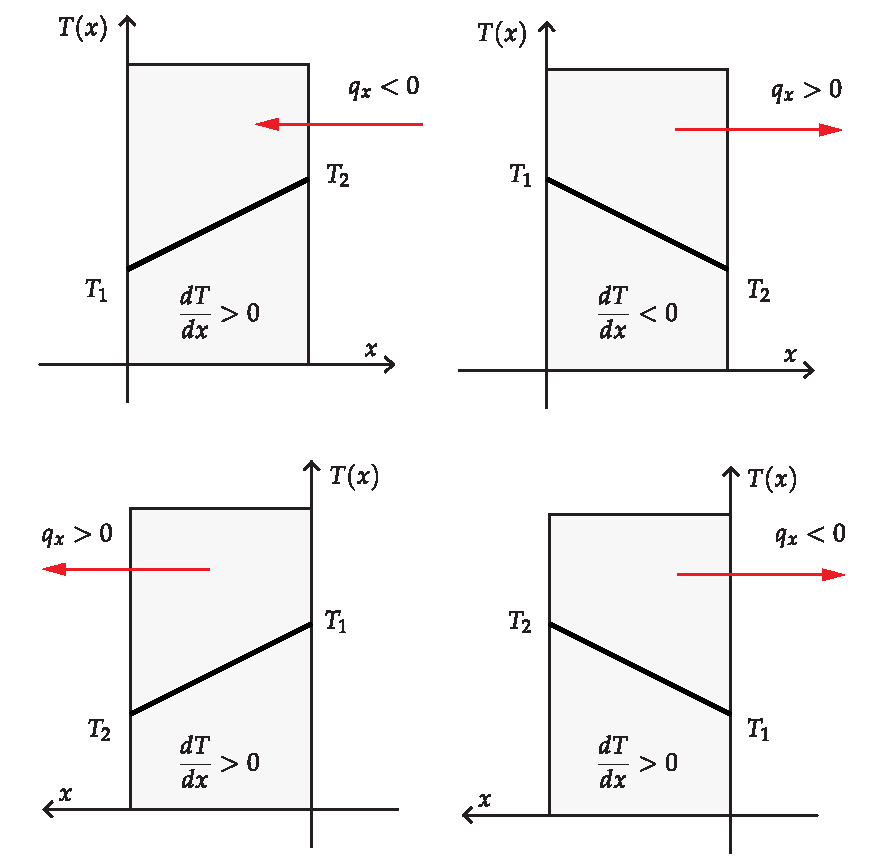
\includegraphics[scale=0.8]{figuras/cap1/fluxo.pdf}
\caption{Convenção do sinal negativo da Lei de Fourier, mudar o sinal da derivada na terceira figura}
\label{fig:sinal}
\end{figure}

Assim, o sinal $-$ é imposto na lei de Fourier para tornar o fluxo de calor uma quantidade positiva na direção da coordenada positiva (ou seja, oposta ao gradiente de temperatura).

Determinar a direção real do fluxo de calor é muitas vezes trivial para problemas unidimensionais (1D). Problemas multidimensionais e notavelmente problemas transitórios, podem apresentar dificuldade considerável em determinar a direção dos termos de fluxo de calor local. Adesão à convenção de sinais para a Lei de Fourier evitará tais dificuldades de determinação de fluxo, o que é útil na contexto de conservação geral de energia para um determinado problema de transferência de calor.

\subsection{Condutividade Térmica}
Dada a dependência direta do fluxo de calor na condutividade térmica via Lei de Fourier, a condutividade térmica é uma propriedade importante na análise da condução de calor. Existe uma ampla variedade de condutividades térmicas de vários
materiais de engenharia. Geralmente, os valores mais altos são observados para metais puros e os menores valores por gases e vapores, com os materiais isolantes amorfos e líquidos inorgânicos com condutividades térmicas intermediárias. 

Para fornecer uma noção da ordem de grandeza da condutividade térmica de diferentes materiais, a Figura \ref{fig:escalacondutividade} apresenta a faixa típica de valores para diversos materiais.

\begin{figure}[H]
\centering
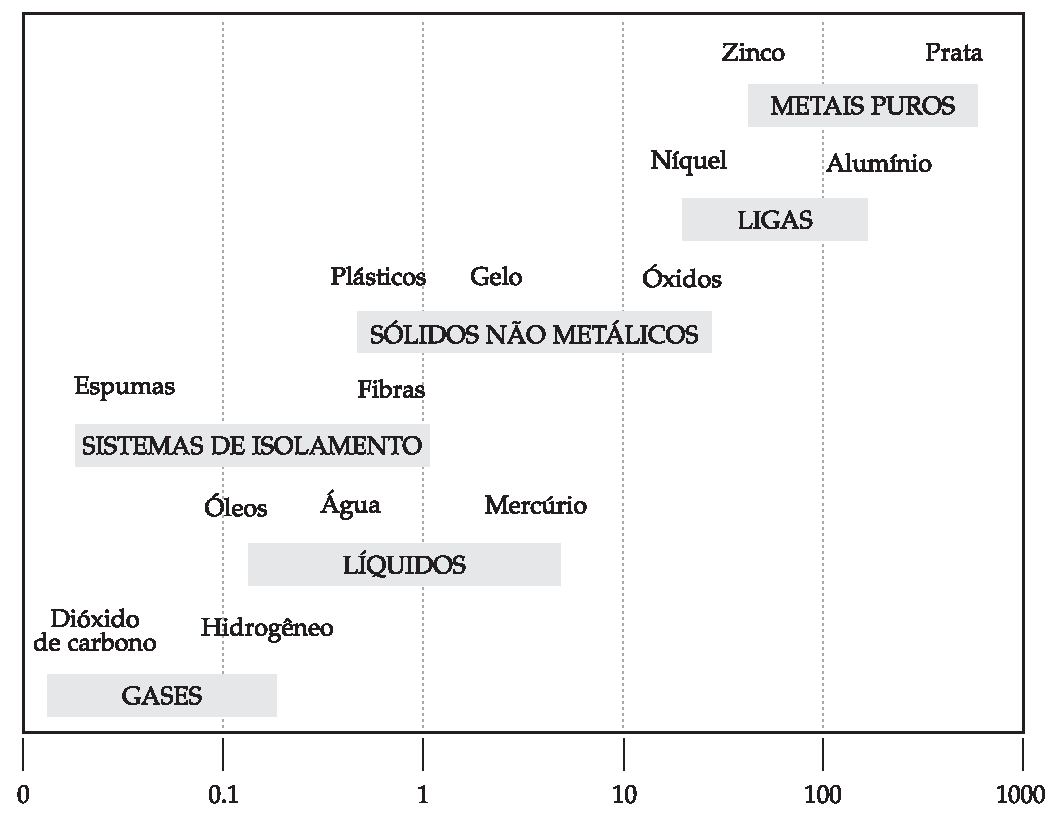
\includegraphics[scale=1]{figuras/cap1/condutividade.pdf}
\caption{Condutividade térmica ($W/mK$), adaptado Incropera.}
\label{fig:escalacondutividade}
\end{figure}

A condutividade térmica também varia com a temperatura e pode mudar com orientação para materiais não isotrópicos. Para a maioria dos metais puros, a condutividade térmica diminui com o aumento da temperatura, enquanto para os gases ela aumenta com o aumento da temperatura. Para a maioria dos materiais isolantes aumenta com o aumento temperatura. 

Uma compilação abrangente de condutividades térmicas de materiais pode ser encontrada nas referências \textcite{arpaci1966, ozisik1993}.

\printbibliography[heading=subbibliography]
